Der findes mange online systemer som tager sig af at udbyde små og store opgaver for forskellige interresenter. Det er blandt andet programmører og grafiske designere der påtager sig opgaver fra disse sites. Dette kan der være flere årsager til. For det første tjener de en skilling på disse opgaver, såfremt de er løst tilstrækkeligt. For det andet får de god erfaring, hvilket også fører til et forbedret CV.\\
\\
En af disse tjenester hedder MTurk, som står for Amazon Mechanical Turk. Systemet er lavet af den multinationale virksomhed Amazon, som mest er kendt for sin store onlineshop. Tjenesten beskriver sig selv som et markedsplads for arbejde som kræver menneskelig intelligens.\cite{MTurk} Den har blandt andet været benyttet af forskere, som har benyttet MTurk's muligheder til at lave større og billigere studier.\cite{Sciencemag} Det fungerer som mange andre freelance systemer, hvor man som arbejder kan vælge mellem en række opgaver, som er blevet opstillet af nogle andre personer. Et eksempel på dette kan ses på figur \ref{MTurkILL}.

\begin{figure}[H]
\centering
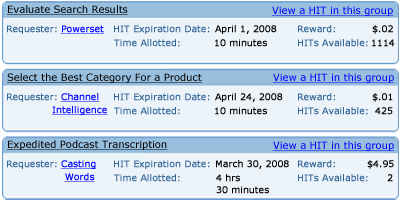
\includegraphics[width=0.6\textwidth]{Billeder/MTurk.png}
\caption{Billedet viser et eksempel på en række opgaver. Billede taget fra mturk.com\cite{MTurkIMG}}
\label{MTurkILL}
\end{figure}

Opgaverne er meget forskellige i hvor meget der kræves af arbejderen og derfor også størrelsen på betalingen, arbejderen får for sit arbejde. Efter man har påtaget sig en opgave, har man så en deadline, inden det udførte arbejde skal være lavet, og afleveret til systemet igen. Herefter vil ens arbejde blive vurderet, og hvis det accepteres vil man få udbetalt et beløb til sin virtuelle konto i systemet. Dette virtuelle beløb kan så blive udbetalt i form af et gavekort til Amazon’s hjemmeside, dog hvis man er bosiddende i Amerika er det muligt at benytte bankoverførsler, eller checks hvis man bor i Indien.\cite{MTurk2}

Som arbejdsgiver, har man mulighed for at opstille en række indstillinger, som gør det muligt for arbejderne at tilfredsstille ens problemer. Heraf er det blandt andet muligt at vælge antallet af personer, denne opgave skal være tilgængelig for en tidsramme, arbejderne skal klare opgaven inden for, eller en deadline inden opgaven forsvinder.\\
\\
En anden af disse tjenester hedder ShortTask. ShortTask er et system opdelt i to grupper, seekers og solvers, arbejdsgivere og arbejdstagere. Seekers er dem der har en uløst opgave, og solvers er dem der kan løse disse opgaver. ShortTask er altså en form for mellemmand der skaber kontakten mellem disse grupper.

Mange firmaer har så mange små opgaver, at det faktisk er en stor byrde for firmaet, og fordi opgaverne er så små er det simpelthen for dyrt at have egne ansatte til at løse disse. Det er her ShortTask (og andre tjenester) kommer ind i billedet, disse tjenester råder over en gruppe solvers, som relativt hurtigt ville kunne løse firmaets små opgaver, grundet kvantiteten af solvers. Fordelen ved systemet er altså at firmaet både sparer penge og tid. Penge fordi opgaverne har en fast pris uanset hvor meget tid en solver bruger på problemet, og denne pris er ofte på få cent. Tid fordi det ikke er dem selv eller deres egne ansatte der bruger tid på opgaven. Sitet er opbygget meget simpelt og brugervenligt. Når man åbner siden kan man hurtigt, selv uden login, åbne en fane med oversigt over uløste opgaver. En forskel på denne tjeneste og MTurk er at MTurk ikke udbetaler kontanter til alle lande, hvilket denne tjeneste gør. \cite{ShortTask}\\
\\
Grundidéen i de ovenstående tjenester har mange ting til fælles med vores projekt. Seekers og solvers svarer til forældre og børn, opgaverne svarer til pligter og sådan findes der flere eksempler. Eftersom disse systemer ligner vores på mange punkter, vil vi lade os inspirere af hvordan de har løst opgaven med at være et digital mellemled mellem arbejdsgiver og arbejdstager. Det er naturligvis i vores interesse at gøre programmet så brugervenligt som muligt, vi kan altså med fordel lade os inspirere af blandt andet ShortTasks design. Yderligere skal børnene som benytter sig af vores lommepengesystem måske have en form for virtuel konto, ligesom nogle af disse freelance systemer gør brug af. Desuden kan vi overveje hvorvidt vi skal gøre ligesom MTurk, og lade barnet vælge opgaven og så have en deadline til at løse denne, eller om barnet skal løse en opgave og så først bagefter angive i vores program at opgaven er løst.


